\documentclass[11pt]{article}

\usepackage{amsmath}
\usepackage{graphicx}
\usepackage{subcaption}

\newcommand{\numpy}{{\tt numpy}}    % tt font for numpy

\topmargin -.5in
\textheight 9in
\oddsidemargin -.25in
\evensidemargin -.25in
\textwidth 7in

\begin{document}

% ========== Edit your name here
\author{Aobo Yang (ay6gv)}
\title{CS6316: HW6}
\maketitle

\medskip

% ========== Begin answering questions here
\begin{enumerate}

\item
Unsupervised Learning with Clustering

1.3 K-means Clustering

\medskip

Figure \ref{fig:k_means} is the scatter plot of the K-means.

\begin{figure}[!h]
  \centering
  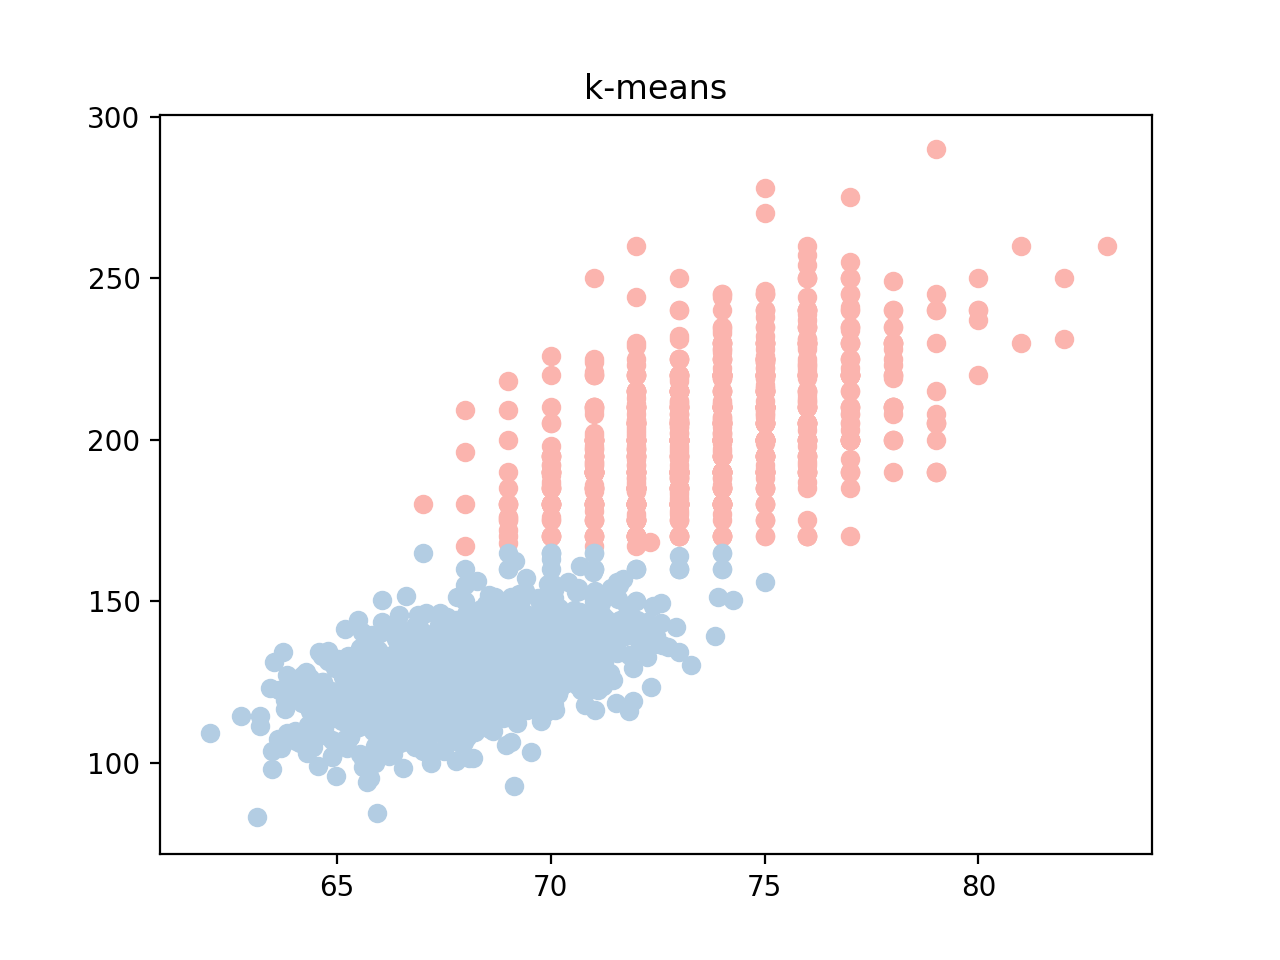
\includegraphics[width=\linewidth]{figures/k_means.png}
  \caption{K-means Scatter Plot}
  \label{fig:k_means}
\end{figure}

The relationship between k and objective function value is shown in Figure \ref{fig:k_knee_finding}.

\begin{figure}[!h]
  \centering
  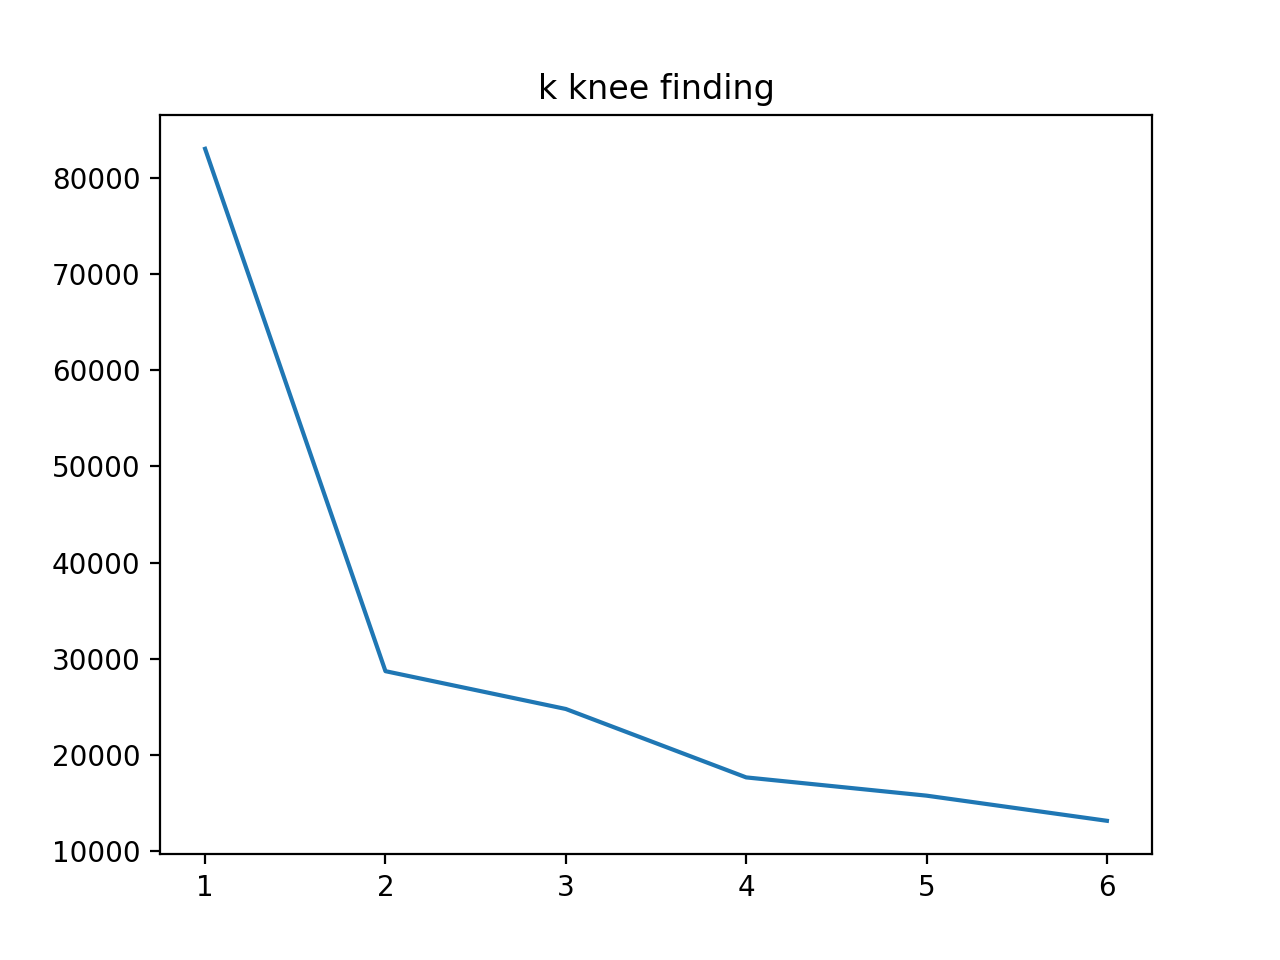
\includegraphics[width=\linewidth]{figures/k_knee_finding.png}
  \caption{K Knee Finding}
  \label{fig:k_knee_finding}
\end{figure}

The purities of clusters when k equals $2$ is shown in the table below

\begin{center}
  \begin{tabular}{ |c|c| }
   \hline
   Cluster & Purity \\
   0 & 0.9990 \\
   1 & 0.9724 \\
   \hline
  \end{tabular}
\end{center}

\medskip

1.4 Guassian Mixture model

Figure \ref{fig:gmm_diag_1} is the scatter plot of the GMM with covType of diag for dataset1.

\begin{figure}[!h]
  \centering
  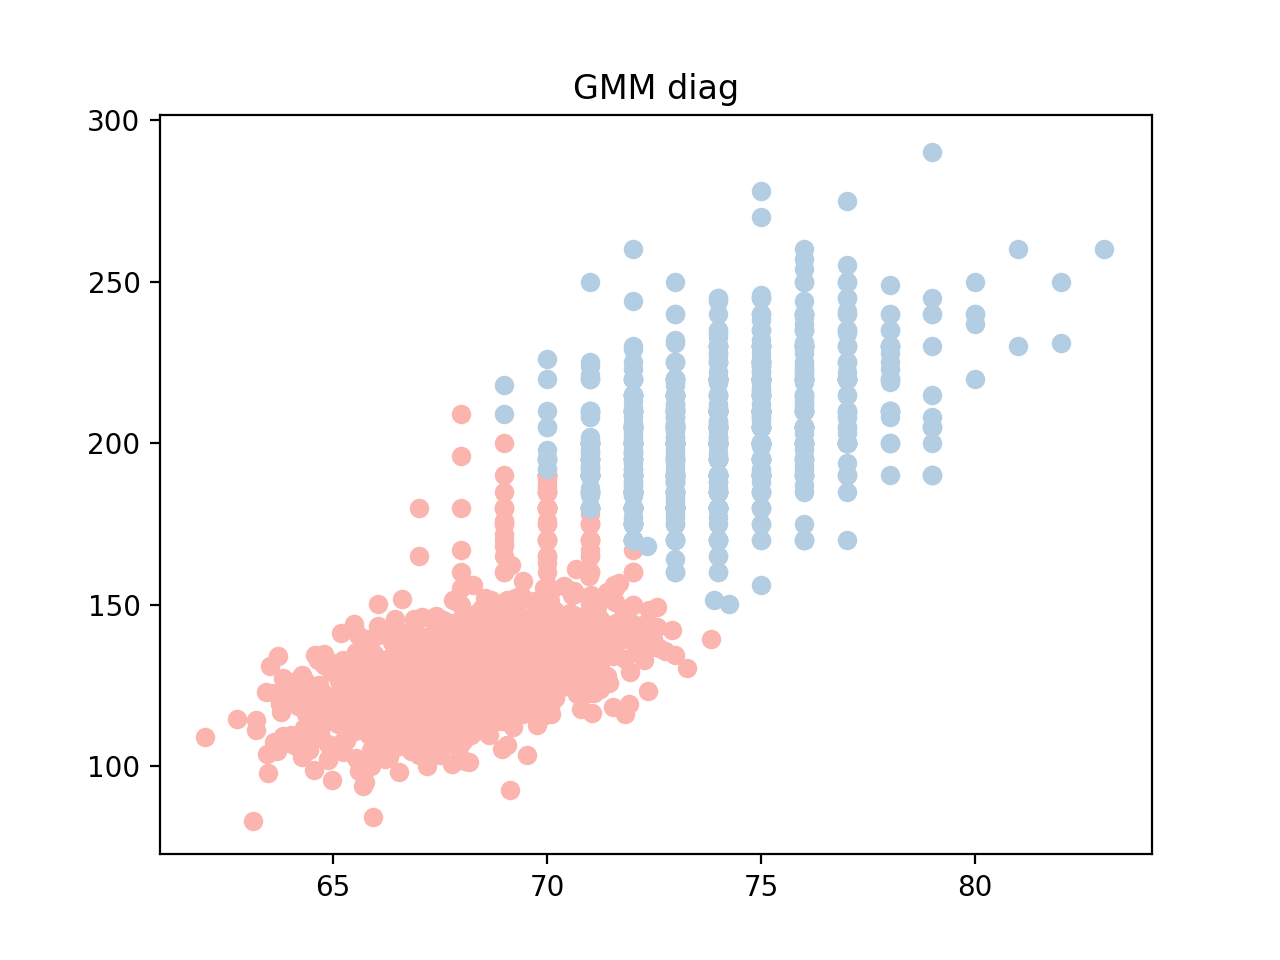
\includegraphics[width=\linewidth]{figures/gmm_diag_1.png}
  \caption{GMM Diag Dataset1 Plot}
  \label{fig:gmm_diag_1}
\end{figure}

Figure \ref{fig:gmm_full_1} is the scatter plot of the GMM with covType of full for dataset1.

\begin{figure}[!h]
  \centering
  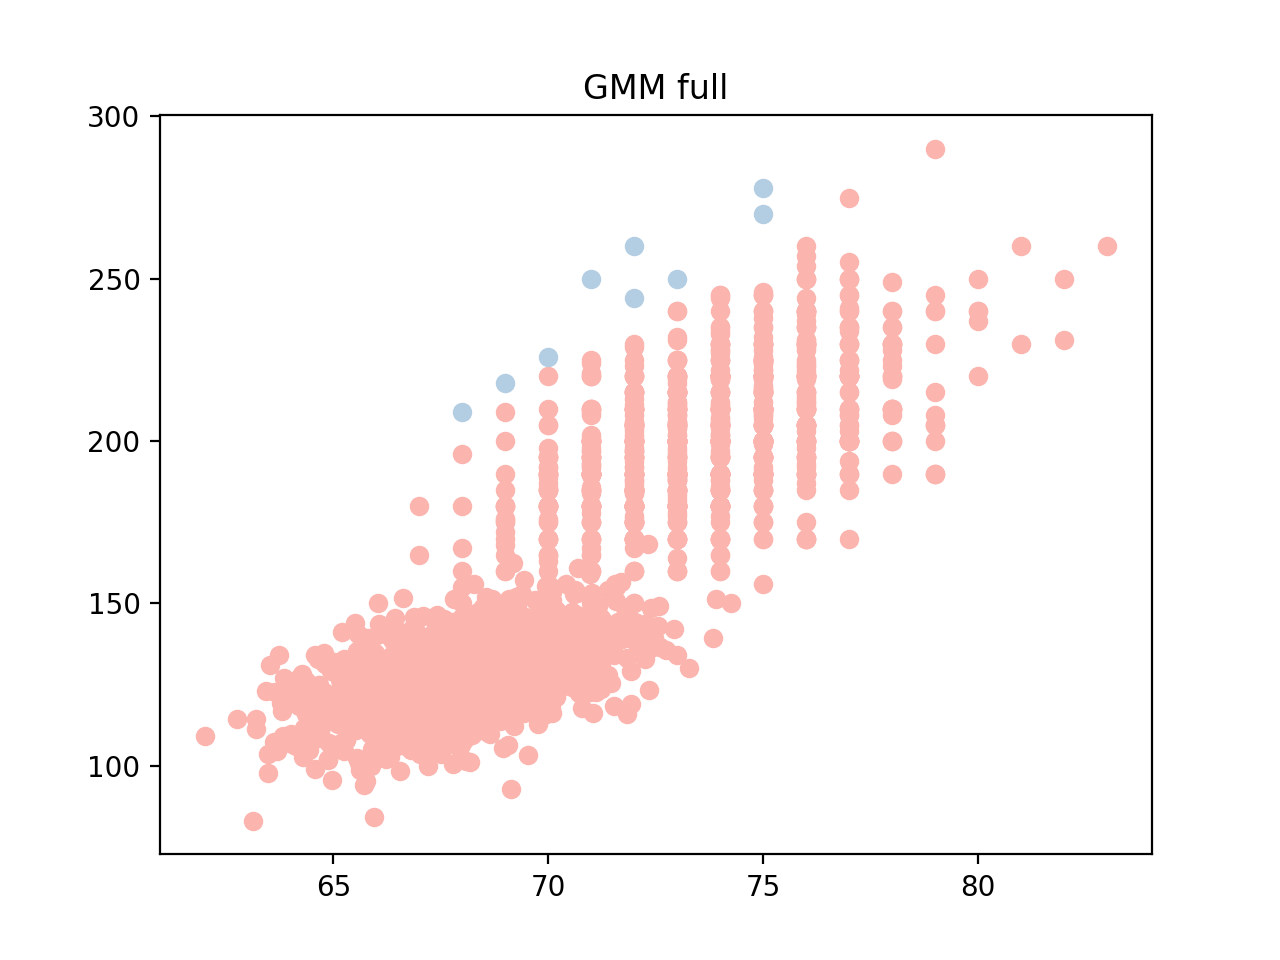
\includegraphics[width=\linewidth]{figures/gmm_full_1.png}
  \caption{GMM Full Dataset1 Plot}
  \label{fig:gmm_full_1}
\end{figure}

Figure \ref{fig:gmm_diag_2} is the scatter plot of the GMM with covType of diag for dataset2.

\begin{figure}[!h]
  \centering
  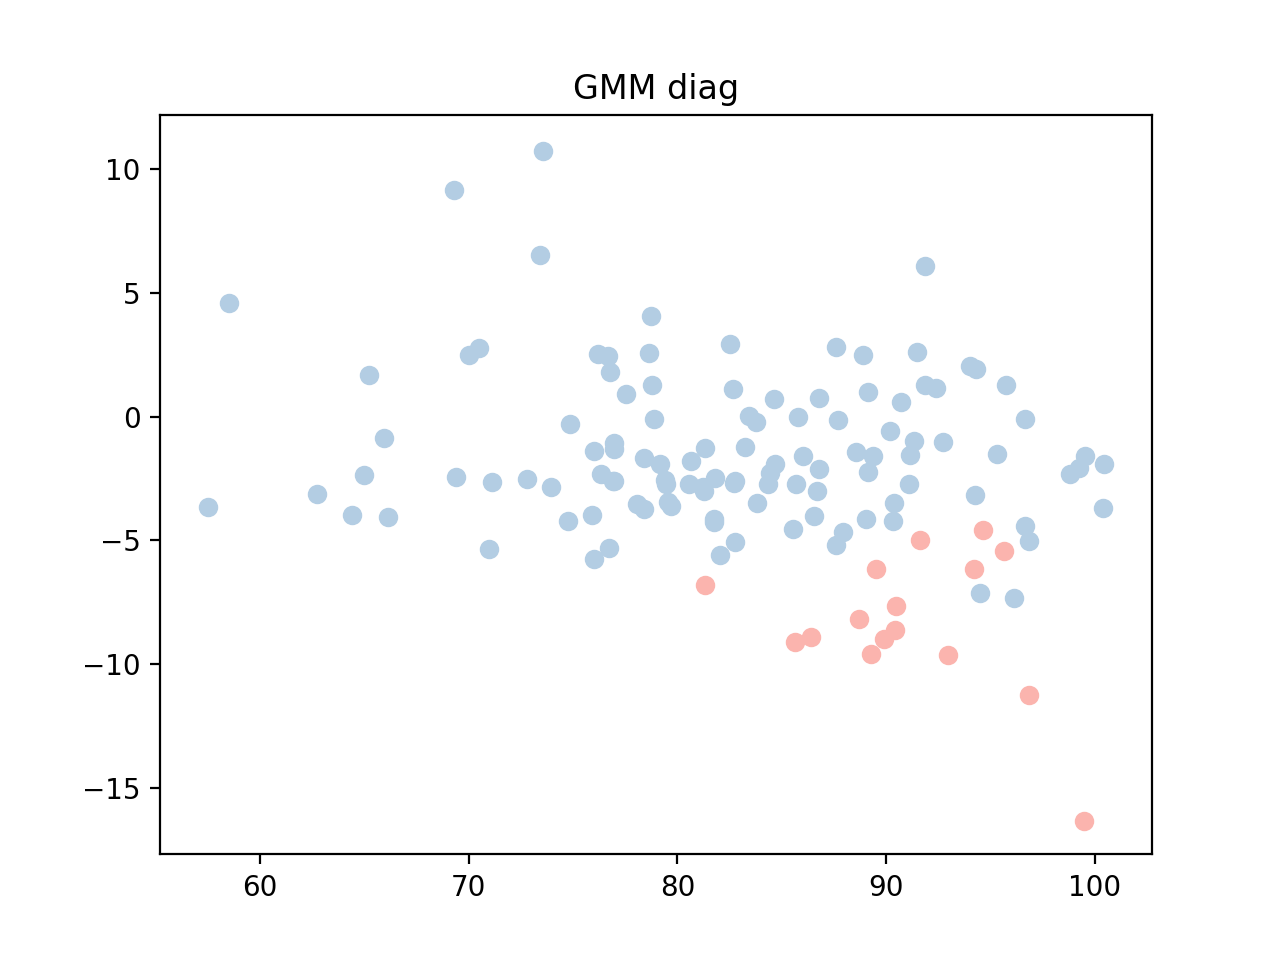
\includegraphics[width=\linewidth]{figures/gmm_diag_2.png}
  \caption{GMM Diag Dataset2 Plot}
  \label{fig:gmm_diag_2}
\end{figure}

Figure \ref{fig:gmm_full_2} is the scatter plot of the GMM with covType of full for dataset2.

\begin{figure}[!h]
  \centering
  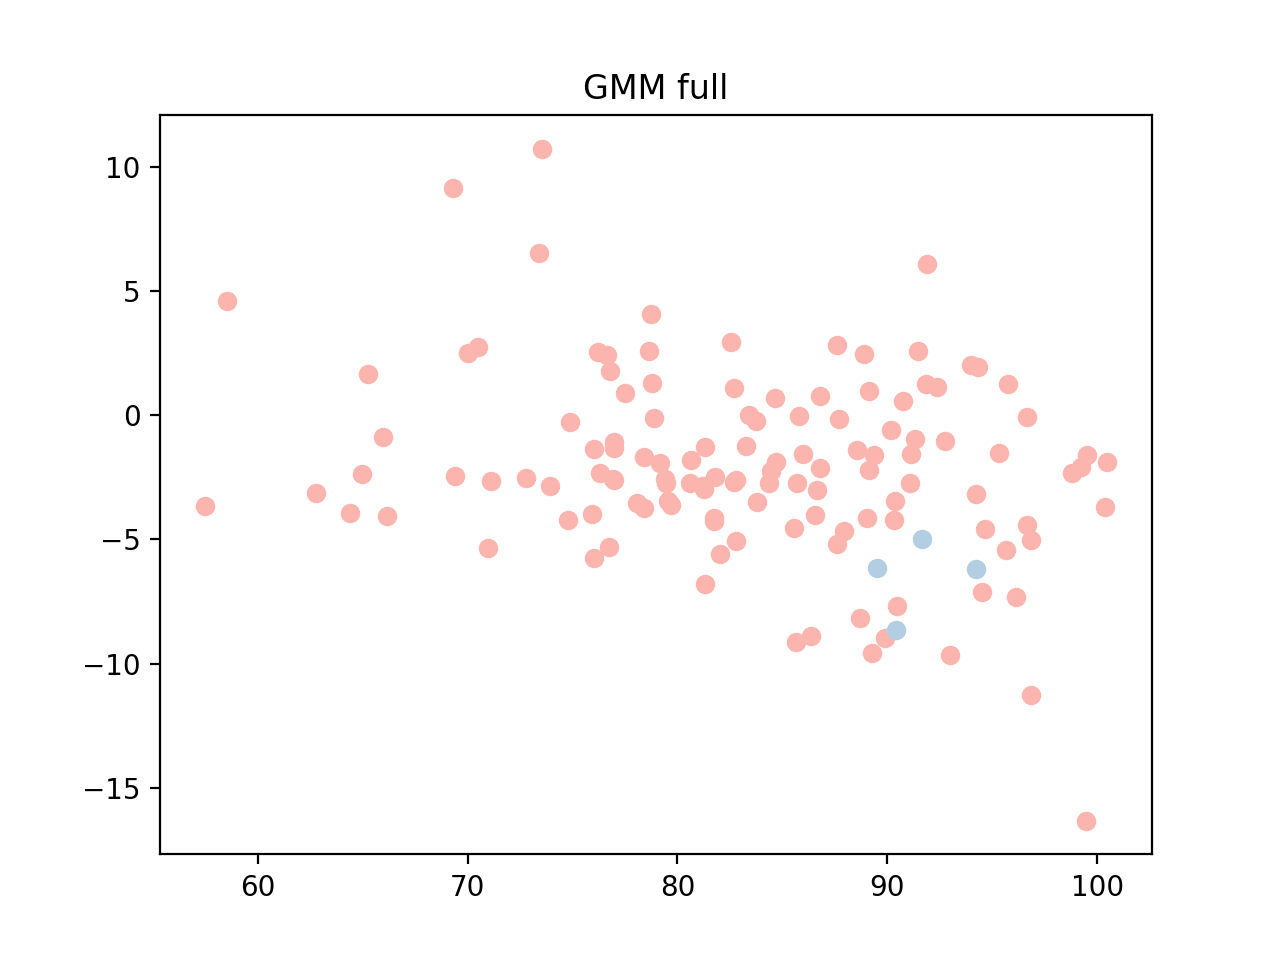
\includegraphics[width=\linewidth]{figures/gmm_full_2.png}
  \caption{GMM Full Dataset2 Plot}
  \label{fig:gmm_full_2}
\end{figure}


The purities of dataset1 with GMM diag are shown in the table below

\begin{center}
  \begin{tabular}{ |c|c| }
   \hline
   Cluster & Purity \\
   0 & 0.9315 \\
   1 & 0.9968 \\
   \hline
  \end{tabular}
\end{center}

The purities of dataset1 with GMM full are shown in the table below

\begin{center}
  \begin{tabular}{ |c|c| }
   \hline
   Cluster & Purity \\
   0 & 1.0 \\
   1 & 0.5394 \\
   \hline
  \end{tabular}
\end{center}

The purities of dataset2 with GMM diag are shown in the table below

\begin{center}
  \begin{tabular}{ |c|c| }
   \hline
   Cluster & Purity \\
   0 & 0.6875 \\
   1 & 0.5268 \\
   \hline
  \end{tabular}
\end{center}

The purities of dataset2 with GMM full are shown in the table below

\begin{center}
  \begin{tabular}{ |c|c| }
   \hline
   Cluster & Purity \\
   0 & 0.5161 \\
   1 & 1.0 \\
   \hline
  \end{tabular}
\end{center}

\item
Sample QA Questions

\medskip

2.2 Decision Tree

\medskip

(a)

$$
-2 * 0.5 * \log_{2}{0.5} = 1.0
$$

\medskip

(b)

$$
- 1 * \log_{2}{1} = 0
$$

\medskip

(c)

$$\begin{aligned}
  H(E|Color) &= p(Color=G)H(E|Color=G) + p(Color=B)H(E|Color=B)\\
  &\; + p(Color=R)H(E|Color=R) \\
  &= 1/3 * 0 + 2/9 * 1.0 + 4/9 * 0 \\
  &= 0.2222
\end{aligned}$$

$$\begin{aligned}
H(E|Wig) &= p(Wig=Y)H(E|Wig=Y) + p(Wig=N)H(E|Wig=N) \\
&= 2/9 * 1.0 + 7/9 * 0.9852 \\
&= 0.9885
\end{aligned}$$

$$\begin{aligned}
  H(E|Ears) &= p(Ears=2)H(E|Ears=2) + p(Ears=3)H(E|Ears=3) \\
  &= 8/9 * 1.0 + 1/9 * 0 \\
  &= 0.8888
\end{aligned}$$

Since the entropy is lowest when conditioned on Color, color will be chosen.

\medskip

(d)

The learned decision tree is shown in Figure \ref{fig:dt}
\begin{figure}[!h]
  \centering
  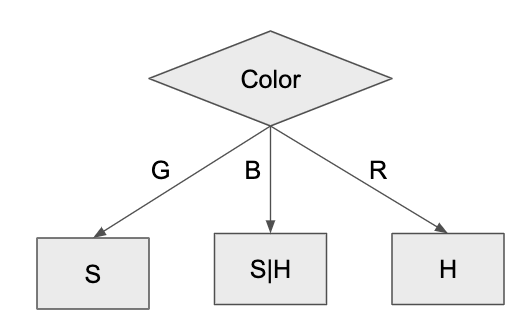
\includegraphics[width=\linewidth]{figures/dt.png}
  \caption{Decision Tree}
  \label{fig:dt}
\end{figure}

\medskip

(e)

The maximum training set error is $$ 50\% $$.

(f)

\begin{center}
  \begin{tabular}{ |c|c| }
   \hline
   Feature 1 & Output \\
   0 & 0 \\
   1 & 0 \\
   0 & 1 \\
   1 & 1 \\
   \hline
  \end{tabular}
\end{center}

% ========== Continue adding items as needed

\end{enumerate}

\end{document}
\grid
\grid
